\begin{frame}[c]{Problema}    
    \begin{minipage}{0.49\textwidth}
        \begin{itemize}
            \item  Grafenas - egzotiška medžiaga, turinti daug pranašumų ir panaudojamumo atvejų.
            \item Bendradarbiavimas su VU Chemijos ir Geomokslų fakulteto mokslininkais.
            \item Grafeno sintezės reakcijos rezultato interpretavimas  prieš įvykdant reakciją.
        \end{itemize}
    \end{minipage}
    \begin{minipage}{0.49\textwidth}
        \begin{figure}
            \centering
            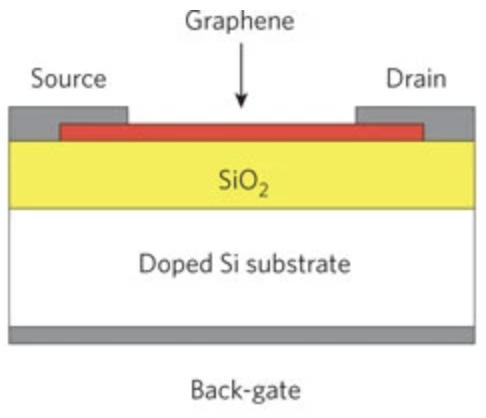
\includegraphics[width=0.5\textwidth]{img/Graphene_MOSFET.png}
            \caption{Grafeno MOSFET tranzistorius \cite{GrapheneMOSFET}}
            \label{fig:graphene_mosfet}
        \end{figure}
    \end{minipage}
\end{frame}